\documentclass[10pt, a5paper]{article}
\usepackage{pdfpages}
\usepackage{parallel}
\usepackage[T2A]{fontenc}
\usepackage{ucs}
\usepackage[utf8x]{inputenc}
\usepackage[polish,english,russian]{babel}
\usepackage{hyperref}
\usepackage{rotating}
\usepackage[inner=2cm,top=1.8cm,outer=2cm,bottom=2.3cm,nohead]{geometry}
\usepackage{listings}
\usepackage{graphicx}
\usepackage{wrapfig}
\usepackage{longtable}
\usepackage{indentfirst}
\usepackage{array}
\newcolumntype{P}[1]{>{\raggedright\arraybackslash}p{#1}}
\frenchspacing
\usepackage{fixltx2e} %text sub- and superscripts
\usepackage{icomma} % коскі ў матэматычным рэжыме
\PreloadUnicodePage{4}

\newcommand{\longpage}{\enlargethispage{\baselineskip}}
\newcommand{\shortpage}{\enlargethispage{-\baselineskip}}

\def\switchlang#1{\expandafter\csname switchlang#1\endcsname}
\def\switchlangbe{
\let\saverefname=\refname%
\def\refname{Літаратура}%
\def\figurename{Іл.}%
}
\def\switchlangen{
\let\saverefname=\refname%
\def\refname{References}%
\def\figurename{Fig.}%
}
\def\switchlangru{
\let\saverefname=\refname%
\let\savefigurename=\figurename%
\def\refname{Литература}%
\def\figurename{Рис.}%
}

\hyphenation{admi-ni-stra-tive}
\hyphenation{ex-pe-ri-ence}
\hyphenation{fle-xi-bi-li-ty}
\hyphenation{Py-thon}
\hyphenation{ma-the-ma-ti-cal}
\hyphenation{re-ported}
\hyphenation{imp-le-menta-tions}
\hyphenation{pro-vides}
\hyphenation{en-gi-neering}
\hyphenation{com-pa-ti-bi-li-ty}
\hyphenation{im-pos-sible}
\hyphenation{desk-top}
\hyphenation{elec-tro-nic}
\hyphenation{com-pa-ny}
\hyphenation{de-ve-lop-ment}
\hyphenation{de-ve-loping}
\hyphenation{de-ve-lop}
\hyphenation{da-ta-ba-se}
\hyphenation{plat-forms}
\hyphenation{or-ga-ni-za-tion}
\hyphenation{pro-gramming}
\hyphenation{in-stru-ments}
\hyphenation{Li-nux}
\hyphenation{sour-ce}
\hyphenation{en-vi-ron-ment}
\hyphenation{Te-le-pathy}
\hyphenation{Li-nux-ov-ka}
\hyphenation{Open-BSD}
\hyphenation{Free-BSD}
\hyphenation{men-ti-on-ed}
\hyphenation{app-li-ca-tion}

\def\progref!#1!{\texttt{#1}}
\renewcommand{\arraystretch}{2} %Іначай формулы ў матрыцы зліпаюцца з лініямі
\usepackage{array}

\def\interview #1 (#2), #3, #4, #5\par{

\section[#1, #3, #4]{#1 -- #3, #4}
\def\qname{LVEE}
\def\aname{#1}
\def\q ##1\par{{\noindent \bf \qname: ##1 }\par}
\def\a{{\noindent \bf \aname: } \def\qname{L}\def\aname{#2}}
}

\def\interview* #1 (#2), #3, #4, #5\par{

\section*{#1\\{\small\rm #3, #4. #5}}

\def\qname{LVEE}
\def\aname{#1}
\def\q ##1\par{{\noindent \bf \qname: ##1 }\par}
\def\a{{\noindent \bf \aname: } \def\qname{L}\def\aname{#2}}
}

\begin{document}
\title{DevOps для QA на примере Java Enterprise проекта\footnote{\url{garanin@itworks.by}, \url{https://www.linkedin.com/in/garaninromanbrest/}, \url{skype://garanin.roman.brest}, \url{https://lvee.org/en/abstracts/284}}}
\author{Гаранин Роман, руководитель отдела тестирования\\ ООО <<Итворкс>>, г. Брест, Беларусь}
\maketitle
\begin{abstract}
In this report, I would like to share the experience of using the DevOps philosophy in our company for one of the projects in the financial sphere. Emphasis will be placed on the work of the quality assurance department, because exactly because of the large number of questions there and the increased quality requirements, the philosophy of DevOps was applied there in the first place.
\end{abstract}
В этом докладе хотел бы поделиться опытом применения философии DevOps: инструментов котейнеризации и непрерывного развёртывания в нашей компании для одного из проектов в финансовой сфере. Упор будет сделан именно на работу отдела QA, потому как именно из-за большого количества вопросов и повышенных требований к качеству философия DevOps была применена там в первую очередь.

Также одна из целей данного доклада~--- это получение обратной связи от участников сообщества (критика, комментарии, предложения по оптимизации).

\subsection*{1. Постановка задачи и описание тестируемого проекта}

Реальный проект большой и сложный, но для лучшего понимания ситуации представим, что у нас имеется портал для  выдачи займов физическим лицам: проверка возможности выдачи займа, оформление соответствующих документов и сопутствующие задачи. Пользователи/клиенты работают с порталом через браузер.

Проект представляет собой J2EE решение, которое состоит из компонентов:

\begin{itemize}
  \item два сервера приложений JBoss (бэк-сервер и фронт-сервер)
  \item ядро системы на Java
  \item процессная часть на JBoss JBPM, куда вынесены бизнес"=процессы
  \item отчеты (JasperReports)
  \item пользовательские формы для отображения в браузере
  \item коннекторы к другим компонентам инфраструктуры (базы данных, сервисы и проч.)
  \item файлы настроек
  \item и многое другое\ldots{}
\end{itemize}

Используемая база данных: Oracle 11g (используется у заказчика).
Исходные коды проекта хранятся в системе контроля версий Mercurial.

Два сервера приложений проекта это:

\begin{itemize}
  \item бэк-сервер~--- с ним работают специалисты заказчика;
  \item фронт-сервер~--- с ним работают клиенты заказчика (через браузер или через мобильное приложение).
\end{itemize}

Упрощенная архитектура тестируемого приложения представлена на рис.~\ref{Gagarin1}:

\begin{center}
\begin{figure}[h!]
  \centering
  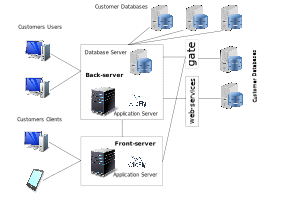
\includegraphics[width=7cm]{13_2018_Gagarin1}
  \caption{~}
  \label{Gagarin1}
\end{figure}
\end{center} 

Началось всё с того, что была поставлена задача по организации автоматических прогонов тестов (GUI) на проекте перед отправкой доработок заказчику. В ходе реализации выяснилось, что и исследовательское (ручное) тестирование также всё еще отнимает много времени и содержит много ручных повторяющихся действий, которые можно оптимизировать. Эти же причины стали препятствием на пути организации автоматизированного тестирования.

Цели, которые мы ставили:

2. Освободить сотрудников от рутинной подготовительной работы и дать им возможность сосредоточиться на задаче.

1. Организовать автоматическое выполнение тестов и быструю обратную связь от процесса развёртывания ПО в тестовой среде.

То есть начали делать цель 1, но пришли к тому, что приоритетнее цель 2 и без реализации цели 2 невозможно реализовать цель 1.

Основной болью сотрудников отдела QA была установка обновлений по доработкам: у каждого специалиста по тестированию были свой сервер JBoss на рабочей машине под Windows и общая база Oracle для тестирования на несколько специалистов. Такой подход приносил целый ряд проблем:

\begin{itemize}
  \item на одной общей базе одни доработки могли ломать другие;
  \item одному тестировщику нужны одни настройки, другому~--- другие, и вот так вот они перетирали друг друга;
  \item если тестировщик не тестировал какое-либо требование, то мог просто не знать об изменениях в некоторых процессах, коннекторах, формах, которые были в работе у другого тестировщика~--- в итоге получали проблему нарушения зависимостей;
и многое-многое другое\ldots{}
\end{itemize}

К тому же ситуация была такова, что при ручном тестировании значительная часть времени тратилась на <<что-то тут недонастроено>>, чем на тестирование нового функционала.

\subsection*{2. Инфраструктура DevOps}

Для решения всех этих проблем была подготовлена инфраструктура. В силу ряда причин (безопасность, конфиденциальность и проч.) решение не вынесено в облака, а полностью находится в локальной сети организации-разработчика. Упрощенно схема показана на рис.~\ref{Gagarin2}:

\begin{center}
\begin{figure}[h!]
  \centering
  \includegraphics[width=7cm]{13_2018_Gagarin2}
  \caption{~}
  \label{Gagarin2}
\end{figure}
\end{center} 

Рассмотрим ее подробнее.

Центральным звеном инфраструктуры является сервер CI под управлением OpenSUSE Linux, на котором установлен Docker. Весь основной софт (который мы рассмотрим ниже) работает в Docker-контейнерах.

Также на сервере CI запущен локальный реестр образов, откуда по сети забираются образы Docker.

Jenkins (Master) следит за обновлениями образов в репозитории Mercurial.

Кроме этого на сервере установлено различное вспомогательное ПО: база MySQL для нужд DevOps, Nginx для публикации отчетов, вспомогательные сервера Mercurial и многое другое. Надо отметить, что новое ПО на CI-сервер устанавливается лишь в крайнем случае~--- всё новое ПО выносится по возможности в контейнеры Docker~--- это очень упрощает дальнейшее сопровождение основной системы и образов.

Частями инфраструктуры также являются:

\begin{itemize}
  \item другие сетевые машины на CentOS для нужд тестирования и отладки, а также по настоящему <<физическая>> машина для запуска тестов мобильного приложения (так как эмуляторы Android не работают на виртуальных машинах);
  \item сетевые базы Oracle 11g для отладки.
\end{itemize}

Рабочее место специалиста по тестированию включает следующее обязательное ПО:

\begin{itemize}
  \item Docker Toolbox~--- набор инструментов для возможности запуска Docker на Windows 10;
  \item Oracle 11g Express Edition~--- локальная база для тестирования, то есть вместо общей сетевой базы у каждого тестировщика появилась своя собственная база, где настройки никто не мог поломать;
  \item Клиент Hg/Mercurial для работы с репозиторием.
\end{itemize}

В Docker-контейнере QA-специалиста запущен Docker-образ с OpenSUSE Linux, где и работает тестируемое приложение.

\subsection*{3. Контейнеризация}

Как было отмечено выше~--- всё основное ПО располагается в контейнерах Docker. Причем в образы кроме тестируемого приложения помещено различное вспомогательное ПО. Это удобно тем, что любой специалист может забрать на свою машину из образа готовое к использованию ПО со всеми настройками.

Организовано это следующим образом: сначала был разработан базовый образ (назовём его itw\_base), который включает минимально необходимое для работы ПО. На основе базового образа строятся другие образы. Для сокращения времени сборки наборы ПО были организованы в промежуточные образы. В результате получилась иерархия, которая упрощенно представлена на рис.~\ref{Gagarin3}:

\begin{center}
\begin{figure}[h!]
  \centering
  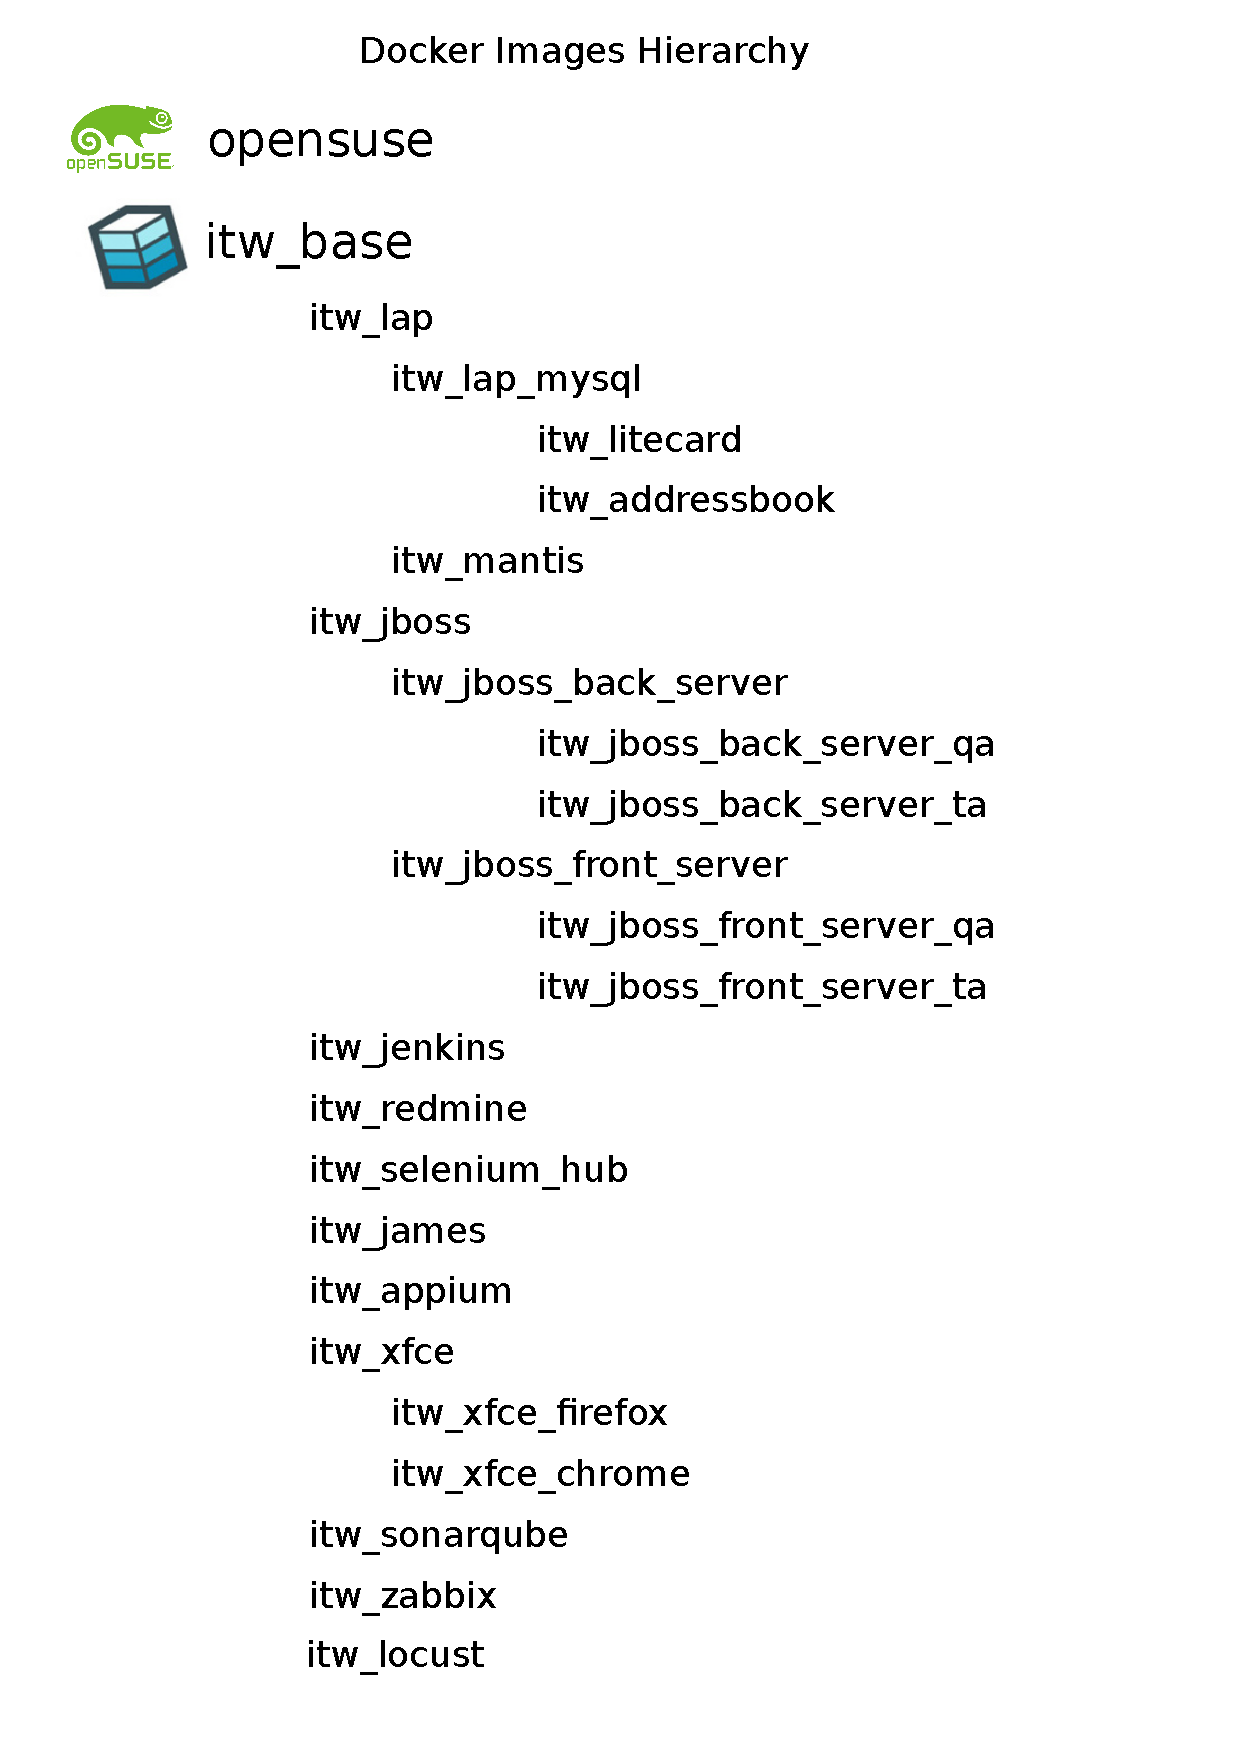
\includegraphics[width=7cm]{13_2018_Gagarin3}
  \caption{~}
  \label{Gagarin3}
\end{figure}
\end{center} 

Базовым Docker-образом является образ itw\_base. Он основан на Docker-образе OpenSUSE.

Сокращенный вариант Dockerfile с комментариями для образа itw\_base приведен по адресу \url{https://bit.ly/2LLX6j6}.

Приведенный Dockerfile не претендует на оптимальность. Его конечно можно оптимизировать, как минимум если уменьшить количество слоёв, но в рамках локальной сети это не сильно критично: все компоненты берутся из текущей папки с Dockerfile или из локальной сети.

При сборке данного образа скрипт zypper\_install\_from\_txt.sh берет построчно содержимое файла base.txt и производит установку необходимого ПО.

Сокращенное содержимое файла base.txt (то есть по сути itw\_base включает в себя перечисленное в файле ПО) можно посмотреть по адресу \url{https://bit.ly/2vvI5qW}.

Таким образом мы получаем готовый и удобный базовый образ, в котором точно есть vim, mc, сервер SSH. Одно из удобств состоит в том, что при подготовке нового образа мы можем развернуть базовый образ на рабочей машине, выполнить установку необходимого нам ПО, провести его настройку, испытания и уже затем приступить к подготовке Dockerfile на его базе.

Пример Dockerfile для дочернего образа можно посмотреть по адресу \url{https://bit.ly/2OBNZ2b}.

Все файлы Dockerfile также лежат в репозитории Mercurial. При коммите в этот репозиторий Jenkins Master начинает пересборку образов, причем он пересобирает образы только по иерархии. То есть если изменения касались промежуточного образа, то пересобираться будет промежуточный образ и его дочерние~--- другие образы затронуты не будут. Скрипт пересборки написан на Groovy и анализирует контрольную сумму в директории с файлом Dockerfile и вспомогательными файлами для сборки. Если контрольная сумма файлов в репозитории стала отличаться, то для этих образов производится пересборка. Такой подход в разы сокращает время на пересборку образов после изменений.

Если изменения коснулись образа itw\_base, то все дочерние образы пересоберутся с этим изменением.

Структура иерархии описана в файле json, пример которого можно посмотреть по адресу \url{http://bit.ly/2vbf8kq}.

\subsection*{4. Continuous Integration (CI)}

Первым делом на Gradle был написан скрипт, который собирает ядро системы. До этого ядро системы мог собрать только разработчик с помощью среды разработки. Причем чтобы собрать ядро ему нужно было прервать текущую работу,  переключить ветки репозитория таким образом, чтобы его работа не затёрлась, собрать ядро, передать его тестировщику, потом переключить ветки обратно и продолжить работу над текущей задачей.

Скрипт сборки на Gradle тестировщик может запустить в любой момент самостоятельно не прибегая к среде разработки (которая при запуске солидно жрёт память) и не отвлекать при этом разработчика.
Этот же скрипт используется для непрерывного развёртывания.

Структура CI представляет собой несколько серверов Jenkins (точнее два сервера). Каждый из них выполняет свою определённую задачу. Все они работают каждый в своём контейнере Docker.

Структура серверов Jenkins представлена на рис.~\ref{Gagarin4}:

\begin{center}
\begin{figure}[h!]
  \centering
  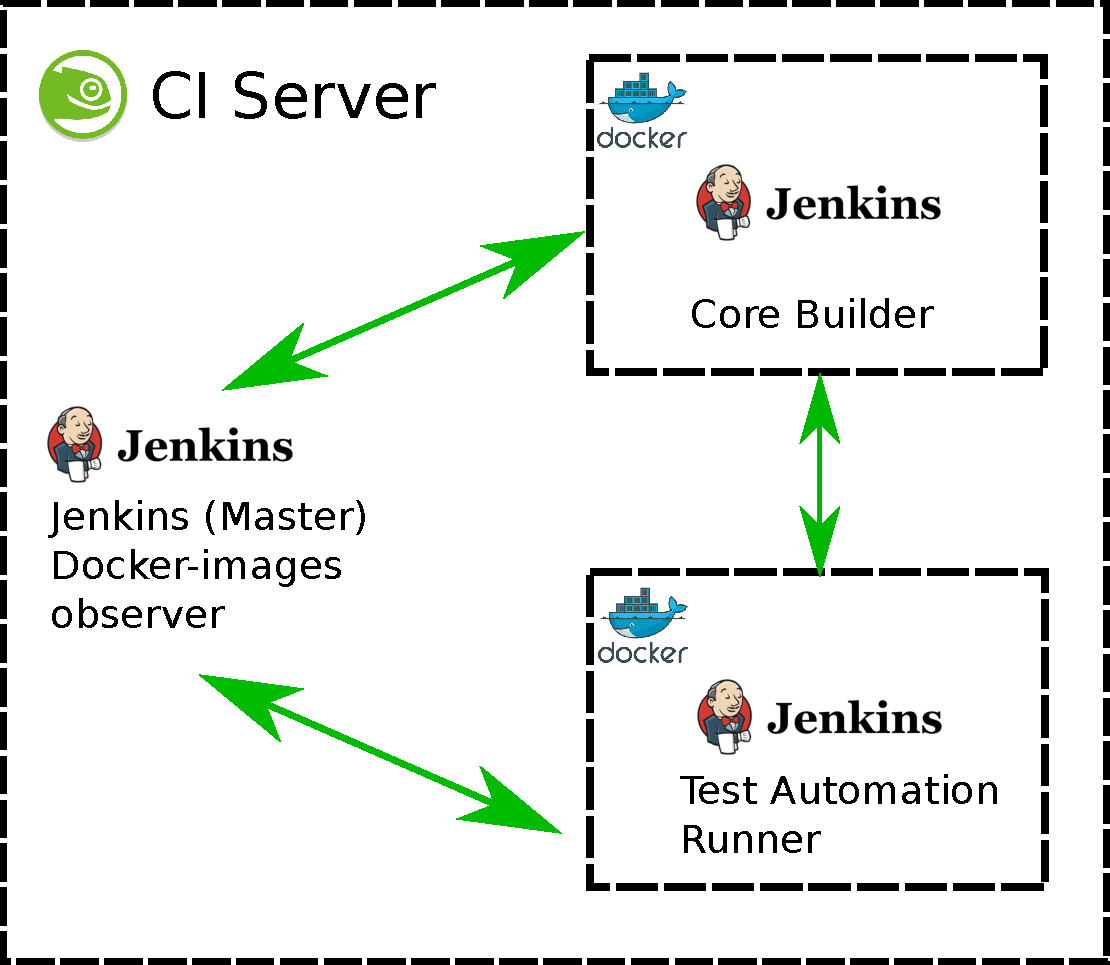
\includegraphics[width=7cm]{13_2018_Gagarin4}
  \caption{~}
  \label{Gagarin4}
\end{figure}
\end{center} 

В этой структуре сервер Jenkins Core Builder, который отвечает за сборку ядра, опрашивает репозитории с исходными кодами проекта. Когда в репозиторий в определенную ветку пришли изменения, то Jenkins производит сборку ядра, запуская скрипт Gradle для сборки.

Если сборка прошла успешно, то управление передается на\\ Jenkins Master, который из образа готовит контейнер для размещения приложения и дальнейшего его тестирования. На этом этапе также производится тестирование сборки контейнера, так как по окончании тестирования этот контейнер (уже протестированный) будет доступен тестировщику на локальной машине из реестра Docker.

Когда контейнер стартовал, то из образа в нем будет размещено и запущено приложение со всеми настройками.

После этого этапа управление передаётся на Jenkins Test\\ Automation Runner, который:

\begin{enumerate}
  \item запускает развёртывание чистой базы данных для теста;
  \item анализирует логи развёртывания базы (устанавливает все апдейты по проекту; если апдейт ошибочный, то тест будет провален);
  \item запускает JBoss сервер приложений;
  \item запускает набор <<дымовых>> браузерных тестов через Selenium Grid;
  \item анализирует логи прогона тестов;
  \item выполняет другие тестовые операции;
  \item отправляет отчет на Jenkins-инициатор.
\end{enumerate}

Результат всех выполненных шагов, также отчет Allure о прогоне тестов, рассылается в виде отчета в Jabber всем заинтересованным участникам: разработчикам, тестировщикам, инженерам DevOps.

Jenkins Test Automation Runner доступен как отдельный настроенный образ, который каждый разработчик/тестировщик может забрать себе на рабочую машину и запустить необходимый набор тестов для проверки регресса или замеров производительности.

Примерный набор тестов Jenkins TA приведён на рис.~\ref{Gagarin5}:

\begin{center}
\begin{figure}[h!]
  \centering
  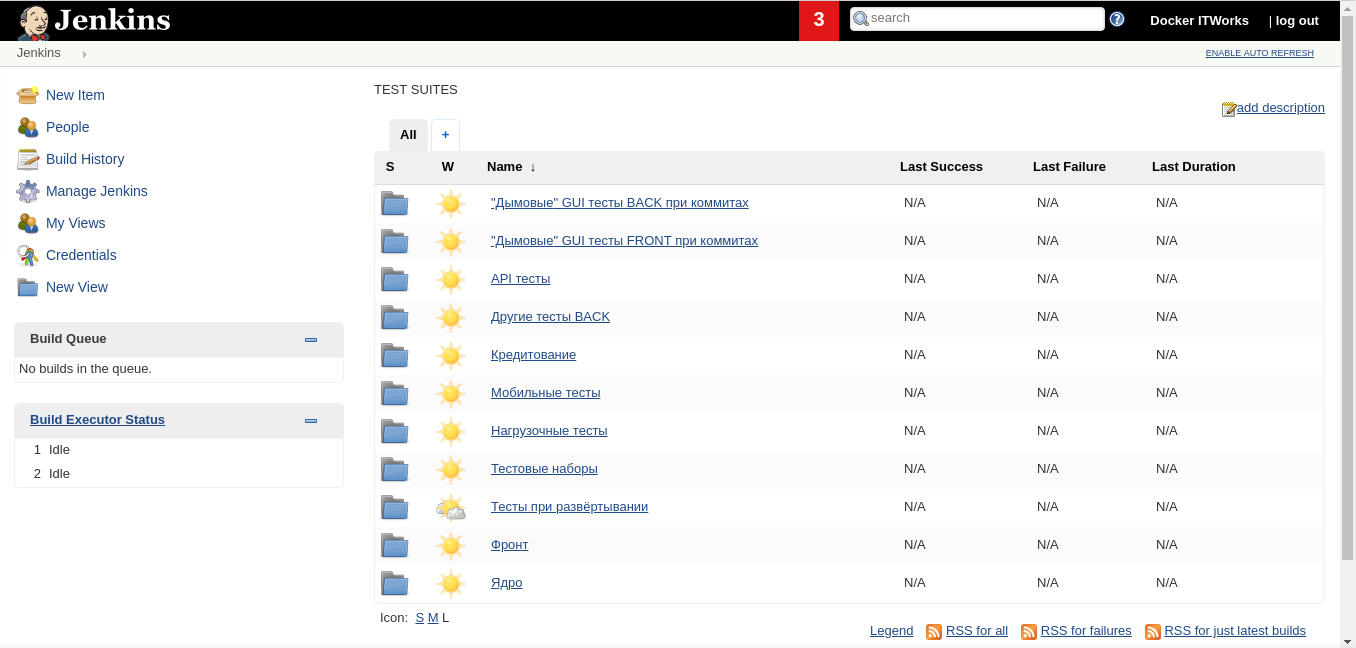
\includegraphics[width=7cm]{13_2018_Gagarin5}
  \caption{~}
  \label{Gagarin5}
\end{figure}
\end{center} 

Для обмена сообщениями между Jenkins'ами используется \\Jenkins REST API.

При коммитах, разумеется, запускается минимальный набор тестов (<<дымовые>> тесты) для получения максимально быстрой обратной связи. Но также возможен запуск и более длительных по времени регрессионных тестов. Для этих целей используются независимые сервера на CentOS из рис. 2: они не зависят от коммитов в репозиторий, и тесты на них могут выполняться несколько часов.

Результирующие отчеты Allure о тестировании помещаются на CI-сервер и доступны всем для ознакомления. Пример такого отчета можно посмотреть здесь: \url{https://demo.qameta.io/allure/latest/}.

После успешного прогона тестов Jenkins Master готовит образ Docker для специалистов по тестированию:

\begin{itemize}
  \item удаляет старый образ из реестра;
  \item собирает новый образ с приложением;
  \item размещает его в реестр образов.
\end{itemize}

Новый образ с приложением~--- полностью протестированный~--- готов для загрузки и дальнейшего использования специалистами по тестированию. Он содержит настроенный сервер со всеми артефактами, перечисленными в разделе 1 данной статьи.

В задачу QA специалиста перед началом тестирования новой доработки входит только подготовить локальную базу данных с помощью скрипта развёртывания (точно такого же, какой выполняет на шаге 1 Jenkins Test Automation Runner). Далее он просто размещает обновления от разработчика и приступает к тестированию.

\subsection*{5. Выводы}

Благодаря использованию подходов DevOps, контейнеризации, CI нам удалось существенно сократить время на регрессионное тестирование, сократить время на ручное тестирование QA"=специалистами, сократить время на подготовку тестовой среды, на выполнение других видов тестов и много других разных преимуществ, что привело к сокращению расходов заказчика и улучшению качества ПО.

Полную презентацию по докладу можно посмотреть по адресу \url{http://bit.ly/2LM4L0K}.

\end{document}
